\documentclass[a4paper, 12pt]{article}

\newcommand{\bold}{\textbf}

\usepackage[english]{babel}
\usepackage{amsmath}
\usepackage{tikz}
\usepackage{indentfirst}

\begin{document}

\newcommand{\q2}{\quad\quad}

\title{\Large{\bold{Moontorio}}}
\author{Matei Adriel}
\date {}

\maketitle

\section{Describing a factory}

A factory is made out of machines. A machine is either a provider, a belt or a  consumer. Machines are connected by ports.

\begin{figure}[h]

\begin{equation}
\begin{split}
Machines\ A,\ B,\ C\ &::=\; belt\ p_i\ p_o \\
        &\quad|\quad provider\ p_1,\ p_2,\ ...\ p_n \\
        &\quad|\quad consumer\ p_1,\ p_2,\ ...\ p_n
\end{split}
\end{equation}
\caption{Machines}
\label{Machines}
\end{figure}

We can represent the factory as a directed graph, with the machines being the nodes and the ports being the edges:

\vspace*{20pt}
\begin{figure}[h]
\centering
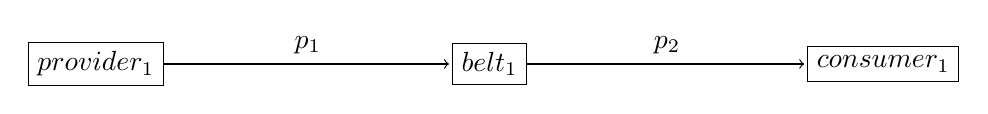
\begin{tikzpicture}[shorten >=1pt, auto, node distance={50mm}, 
  main/.style = {draw, rectangle}]

\node[main] (1) {$provider_1$};
\node[main] (2) [right of=1] {$belt_1$};
\node[main] (3) [right of=2] {$consumer_1$};

\draw[->] (1) edge node{$p_1$} (2);
\draw[->] (2) edge node{$p_2$} (3);

\end{tikzpicture}
\caption{Example of a simple factory} 
\label{SimpleFactory}
\end{figure}

\section{Constraints}
The first step of the factory solving process is the constraint generation. 
We currently use 3 different types of constraints (Figure \ref{Constraints}). 
Let's take them one step at a time. The first two constrains (
  $p_k(t) <_{\Leftarrow} f(t)$ and $p_k(t) <_{\Rightarrow} f(t)$
) are pretty similar, both limiting the flow through a port.

\begin{figure}[ht]

\begin{equation}
\begin{split}
Constraints\quad C_k\ &::=\; p_k(t) <_{\Leftarrow} f(t) \\
        &\quad|\quad p_k(t) <_{\Rightarrow} f(t) \\
        &\quad|\quad p_1(t) = p_2(f(t))  
\end{split}
\end{equation}
\caption{Constraints}
\label{Constraints}
\end{figure}

\end{document}
